\chapter{Literature Review}
\phantomsection
\label{ch:literature}

\section{Khmer Script Overview}
\phantomsection
\label{sec:ocr-overview}
​ ​ ​ ​ The Constitution of Cambodia establishes Khmer as the 
official language, making accurate digital processing of
Khmer documents crucial for national development \citet{Accuracy_Improvement}.



\section{Definition of Optical Character Recognition (OCR)}
\phantomsection
\label{sec:ocr-definition}
​ ​ ​ ​ Optical Character Recognition (OCR) is a field of computer vision and pattern recognition
 that focuses on the automatic identification and digitization of printed or handwritten 
 text from images, scanned documents, or other visual media \citep{singh2012survey}. 
 OCR systems aim to convert visual representations of text into machine-encoded formats, 
 enabling automated indexing, editing, and data extraction \citep{muaz2015khmerocr}.

Modern OCR technology has evolved significantly from its early rule-based and template-matching
roots to incorporate advanced machine learning techniques, particularly deep learning,
which allow for improved accuracy in character detection, segmentation, and classification across 
diverse languages and scripts.

OCR systems typically consist of several key components: image preprocessing (e.g., noise removal, binarization), text detection, character segmentation, feature extraction, and recognition. These systems must be adapted to handle various font styles, image distortions, complex layouts, and script-specific features. While OCR for Latin-based languages has become highly accurate, extending such systems to non-Latin scripts—such as Khmer—remains a significant research challenge due to unique linguistic and structural characteristics.
  

\section{Text Detection}
\phantomsection
\label{sec:text_detection_literature}

  ​ ​ ​ ​  \citet{Hiremath_text_detection} The task of detecting text regions in images is a 
crucial first step in many document analysis pipelines.Character Region Awareness by \citet{Baek}
proposed an efficientand accurate scene text detection approach by incorporating character region 
masking and attention. 

\citet{Hiremath_text_detection} Some other popular research Methodology for text detection and 
highly cited text detection algorithms such as:

EAST (Efficient and Accurate Scene Text Detector) \citet{Zhou} uses a fully convolutionalnetwork to 
directly predict word or text line bounding boxes along with their orientation. 
It was one of the first modern deep learning models for this task. TextBoxes++ \citet{TextBoxes}
extended the TextBoxes model with more powerful convolutional features and anangle 
vector to better handle oriented and curved text instances.  CRAFT (CharacterRegion Awareness for 
Text Detection) \citet{Baek} akes a different approach, using a regionscore map to localize 
individual character regions which are then grouped into words/text lines.
Mask TextSpotter \citet{TextSpotter} combines semantic segmentation + attention-based 
recognition to directly read text of any shape from natural scenes—all in one unified model.
TextFuseNet \citet{ijcai2020p72} is detects text by extracting and fusing features 
at three levels: character-level, word-level, and global-level. It uses a semantic segmentation 
branch for global context, detects characters and words through a modified Mask R-CNN pipeline, 
and combines all levels using a multi-path fusion architecture. This fusion enriches the text 
representation, enabling the model to better localize and segment text instances of arbitrary shapes.
ABCNet \citet{ABCNet} have been proposed which aim to jointly optimize text detection and 
recognition in a unified architecture. Such unified frameworks potentially allow the two tasks 
to benefit from each other during training. 

% Define a custom column type for better control
\newcolumntype{L}[1]{>{\raggedright\arraybackslash}p{#1}} % left-aligned fixed width
\newcolumntype{C}[1]{>{\centering\arraybackslash}p{#1}}   % centered fixed width

\begin{table}[H]
  \centering
  \caption{Text Detection Accuracy}
  \begin{tabularx}{\linewidth}{|L{3.5cm}|L{2.5cm}|L{2.5cm}|C{2cm}|C{2cm}|C{2cm}|}
    \hline
    \textbf{Model} & \textbf{Backbone} & \textbf{Dataset} & \textbf{Recall (\%)} & \textbf{Precision (\%)} & \textbf{F1-score (\%)} \\
    \hline
    EAST* & VGG-16 & ICDAR 2015 & 78.3 & 83.3 & 80.7 \\
    He et al. & ResNet-50 & ICDAR 2015 & 80.0 & 82.0 & 81.0 \\
    R2CNN & VGG-16 & ICDAR 2015 & 79.7 & 85.6 & 82.5 \\
    TextSnake & VGG-16 & ICDAR 2015 & 80.4 & 84.9 & 82.6 \\
    TextBoxes++* & VGG-16 & ICDAR 2015 & 78.5 & 87.8 & 82.9 \\
    EAA & ResNet-50 & ICDAR 2015 & 83.0 & 84.0 & 83.0 \\
    Mask TextSpotter & ResNet-50 & ICDAR 2017 & 81.2 & 85.8 & 83.4 \\
    PixelLink* & VGG-16 & ICDAR 2017 & 82.0 & 85.5 & 83.7 \\
    RRD* & ResNet-50 & ICDAR 2017 & 80.0 & 88.0 & 83.8 \\
    Lyu et al.* & ResNet-50 & ICDAR 2017 & 79.7 & 89.5 & 84.3 \\
    FOTS & ResNet-50 & ICDAR 2017 & 82.0 & 88.8 & 85.3 \\
    CRAFT & VGG-16 & ICDAR 2015 & 84.3 & 89.8 & 86.9 \\
    \hline
  \end{tabularx}
  \caption*{Source: Results sourced from the CRAFT research paper \cite{Hiremath_text_detection}. 
  Results are reported on quadrilateral-type datasets such as ICDAR. 
  Asterisks (*) denote results based on multi-scale tests. 
  The table compares various scene text detection models—including the CRAFT model used in the proposed system—across key performance metrics such as precision, recall, and F1-score.}
  \label{tab:text_detection_accuracy}
\end{table}

\vspace{1em}



\section{Khmer Optical Character Recognition (OCR)}
\phantomsection
\label{sec:khmer_OCR_literature}

​ ​ ​ ​ \citet{CheyFirstOCR} The first significant research on Optical Character Recognition (OCR) 
for Khmer script was proposed in 2006, marking a foundational contribution 
to Khmer language digitization. The study addressed critical challenges 
inherent to Khmer printed characters, notably the variation in character 
shapes across fonts and the high visual similarity between certain 
characters. To overcome these issues, the authors introduced a novel 
recognition method utilizing Wavelet Descriptors. The approach involved 
transforming printed character images into their skeleton forms, 
then converting these skeletons into the temporal domain. Character 
templates were generated using wavelet coefficients from a training set, 
and recognition was performed through a deformable wavelet descriptor 
and a Euclidean distance classifier. The recognition process selected 
the template with the smallest distance to the input character as the 
result. Interestingly, deformation was later excluded from the final 
method due to its adverse impact on distinguishing similar characters. 
Experimental evaluation demonstrated promising results: recognition 
rates of 92.85\%, 91.66\%, and 89.27\% for 22-point, 18-point, and 
12-point font sizes respectively, across 10 Khmer fonts. A second 
test used a 21-page document scanned at varying resolutions 
(150, 300, 600 dpi) and fax inputs, achieving recognition rates 
of 92.99\% at 300 dpi, 88.61\% at 150 dpi, and 80.05\% for faxed documents. 
This pioneering work laid the groundwork for future Khmer OCR systems 
and remains a landmark study in Khmer script recognition.

\citet{Sok&Taing2014} The second significant research on 
Khmer Optical Character Recognition (OCR) introduces a Support 
Vector Machine (SVM)-based approach for printed Khmer character 
recognition in bitmap documents. Given the inherent complexity 
of the Khmer script—which includes 74 alphabets and the potential 
for up to five vertical levels in word compounds—the study focuses 
on identifying the most effective SVM kernel for classification.

The proposed method evaluates three SVM kernels: Gaussian, Polynomial, 
and Linear. Rather than training on large datasets, the system adopts 
a modular approach, segmenting characters into smaller parts. Each 
segment is transformed into a binary matrix, with 1s representing 
black pixels and 0s for whitespace. Feature extraction is applied 
to these matrices for SVM training and classification.

Following recognition, post-processing rules are employed to merge 
character clusters and correct common misclassifications based on 
character levels. The training utilized one font ("Khmer OS Content") 
at 32pt and tested recognition performance across three font sizes 
(28pt, 32pt, and 36pt). The results demonstrated strong accuracy:
\begin{itemize}
  \item 98.17\% for 28pt,
  \item 98.62\% for 32pt,
  \item 98.54\% for 36pt.
\end{itemize}

The Gaussian kernel outperformed the other kernels, confirming its 
suitability for Khmer character recognition. This study highlights 
the effectiveness of machine learning-based OCR for complex scripts 
like Khmer and marks a major advancement over earlier template-based 
systems.

\citet{Meng_Hann_2014} proposed a Khmer Character Recognition (KCR) 
system utilizing artificial neural networks to address the complexity 
of recognizing individual Khmer script characters. Developed in a 
MATLAB environment, the system integrates a Self-Organizing Map (SOM) 
for unsupervised clustering with a Multilayer Perceptron (MLP) 
trained via the backpropagation algorithm for supervised classification. 
The recognition process follows a two-stage pipeline: first, the input 
image—resized to 20×20 pixels—is categorized by the SOM into one of 
nine coarse groups. Then, each group is assigned to a dedicated MLP 
model, which performs fine-grained classification into one of 82 
target classes, including Khmer consonants, vowels, and numerals. 
This modular approach aims to enhance classification efficiency by 
narrowing the decision space for each MLP. The system achieved an 
average recognition accuracy of 65\% on the training dataset and 
30\% on the testing dataset, highlighting both the potential and 
the challenges of neural network-based Khmer OCR at the time.

\citet{Muaz2015} This study presents a comprehensive OCR system for 
printed Khmer text using the HTK Toolkit, covering the full 
pipeline of pre-processing, segmentation, recognition, and mapping. 
The system is tailored for the widely used Limon S1 font at 22pt and 
introduces a structural segmentation approach that decomposes 
characters into five categories: Main Body, SuperScript, SubScript, 
CCDown, and Complex Character (CC). Feature extraction relies on 
vertical framing and Discrete Cosine Transform (DCT), with 
classification handled by Hidden Markov Models (HMMs). 
The system was trained on over 35,000 labeled shape samples and 
evaluated on 10 pages of scanned newspaper text, achieving an 
overall recognition rate of 96.34\%. While the results are promising, 
the system is limited by its reliance on a single font style and size, 
making it less robust to font variation. Additionally, recognition 
performance drops for complex shapes like CC (70.88\%) and depends 
heavily on manually crafted mismatch and rule files for post-processing, 
indicating scalability and generalization challenges for real-world 
applications involving diverse document types and fonts.

\citet{Valy_8563219} proposed a character-level Convolutional Neural 
Network (CNN) model for recognizing ancient Khmer script from digitized 
palm leaf manuscripts. The study focuses on two core tasks: 
isolated character recognition and word-level glyph localization. 
For the character recognition task, a CNN architecture comprising 
three convolutional blocks followed by a linear classifier was 
developed. The output layer of the network predicts one of 106 
character classes, achieving a reported test accuracy of 95.96\%. 
In addition to CNNs, the study also explores other neural 
architectures including LSTM-RNN and hybrid CNN-RNN models. 
For the word/text image recognition task, the authors leveraged 
both one-dimensional and two-dimensional RNNs to handle the complex 
spatial structure of Khmer script and to localize glyphs within 
variable-length text patches. This research highlights the potential 
of deep learning approaches in historical Khmer OCR, particularly in 
handling the challenges posed by degraded manuscripts and complex 
writing structures.

\citet{Annanurov_2018} conducted a pilot study on Khmer handwritten 
symbol recognition, focusing on the use of Convolutional Neural 
Networks (CNNs) for digitizing large-scale handwritten document corpora. 
The study used image data from six handwriting datasets containing 
33 Khmer consonants and 17 vowels, forming a total of 561 syllables. 
For consonant recognition, the authors trained 33 individual CNNs—one 
for each root radical—which were later integrated into a recognition 
assembly. The performance of the CNN-based model was evaluated against 
two alternative systems: an artificial neural network (ANN) using the 
full feature set, and another ANN with reduced feature dimensions. 
Feature extraction techniques such as two-dimensional Fourier 
transformation (FT2D) and Gabor filters were employed for dimensionality 
reduction. The CNN-based approach achieved a recognition accuracy of 
up to 94.85\%, outperforming the ANN-based models. However, the system 
was limited to recognizing only Khmer consonants, without support for 
vowel or syllable-level recognition.

\citet{sokphyrum2019khmer} fine-tuned the Tesseract OCR engine 
(version 4.0) to improve recognition of Khmer Unicode and legacy 
Limon fonts. Tesseract 4.0 employs a deep convolutional recurrent 
neural network with a connectionist temporal classification (CTC) 
loss function and attention mechanism, enabling it to recognize entire 
text-line images. The fine-tuning process involved training on 14 Khmer 
Unicode fonts and 20 pre-Unicode Limon fonts (all at 12pt size). 
The ISRI Analytic Tools were used to evaluate OCR accuracy at both 
the character level (CHL) and cluster level (CLL) by comparing OCR 
outputs to ground truth text. The Khmer pre-trained engine achieved 
an average accuracy of 87.49\% at the character level and 89.43\% at 
the cluster level on Unicode fonts, while legacy Limon fonts yielded 
a significantly lower median accuracy of 62.27\%. After fine-tuning, 
recognition accuracy reached up to 90\% for specific fonts, demonstrating 
the potential of domain-specific adaptation to enhance OCR performance 
for complex scripts like Khmer.


\citet{Buoy2022} Khmer printed character recognition presents significant 
challenges due to the script's complex structure, including stacked consonants, 
dependent vowels, and diacritics placed in various positions. Traditional approaches, 
such as SVMs, wavelet-based templates, and CNNs, have largely focused on recognizing standalone 
characters and depend heavily on accurate segmentation, making them less robust for noisy or 
continuous text-line images. Tesseract OCR, though improved with deep neural networks 
and CTC loss, still performs poorly on heavily augmented images with a reported Character 
Error Rate (CER) of 35.9\%. In contrast, the reviewed study introduces an end-to-end 
attention-based Sequence-to-Sequence (Seq2Seq) model that directly maps entire text-line 
images to character sequences without needing pre- or post-processing. Trained on 3 million 
synthetically generated and augmented images across multiple Khmer fonts, the model 
achieved a CER of 0.7\% on noisy images and 0.24\% on clean images, significantly 
outperforming existing methods and demonstrating the effectiveness of attention mechanisms 
and deep learning for low-resource scripts like Khmer.

\citet{nom2024khmerst} The Khmer script poses significant challenges for scene text detection 
and recognition due to its complex structure involving stacked consonants, multiple diacritics, 
subscript characters, and the lack of explicit word boundaries. To address the scarcity of 
resources for this low-resource language, this study introduces KhmerST, the first annotated 
scene-text dataset for the Khmer language, consisting of 1,544 real-world images captured 
from various public settings in Cambodia. Unlike existing synthetic Khmer datasets, 
KhmerST includes indoor and outdoor images with diverse fonts, orientations, and 
background conditions, and provides polygon-based line-level annotations for more accurate 
localization. Benchmarking with YOLO models shows that YOLOv8 performs best in detection 
tasks due to its ability to handle small and variable text elements, while in recognition 
tasks, both TrOCR and Tesseract perform poorly, with TrOCR achieving CER of 0.90 and 
Tesseract CER of 1.30, highlighting the need for Khmer-specific OCR models. The study 
underscores the gap between current OCR systems and the needs of Khmer script recognition, 
calling for future research on synthetic data generation, Khmer-aware model design, 
and multimodal approaches to improve accuracy in real-world applications.

\citet{Rina2025} This research addresses the challenge of Khmer textline recognition, 
which is particularly difficult due to the absence of spaces between words in the Khmer script. 
Unlike Latin-based languages, this structure requires recognition to be performed at the textline level, 
leading to high latency when using autoregressive (AR) decoders that predict one character at a 
time while considering previous characters. In contrast, non-autoregressive (NAR) decoders can decode 
all characters in parallel but lack awareness of character dependencies, resulting in lower linguistic 
accuracy. To solve this, the authors propose an efficient Khmer textline recognition method using an NAR 
decoder, enhanced by Khmer-specific subword modeling. Instead of predicting single characters, the model 
recognizes character clusters (subwords), capturing the syntactic, morphological, and orthographic 
structure of the language implicitly. This design retains the speed of NAR models while improving accuracy. 
Experimental results show that the proposed method outperforms the character-level NAR baseline 
in accuracy and matches or exceeds the AR baseline while maintaining lower latency. However, 
the abstract does not report detailed accuracy or metrics, and access to full experimental results 
requires a subscription, limiting transparency for non-subscribers. This work contributes an 
important step toward faster and more linguistically aware Khmer OCR by bridging the gap between 
speed and accuracy in scene text recognition.

Khmer OCR research has progressed significantly, yet the script’s structural complexity—including 
stacked consonants, subscript forms, diacritics, and the absence of spaces between words—continues 
to pose major challenges. Early methods relying on wavelet descriptors, SVMs, and HMMs showed moderate 
success but struggled with font variations, segmentation, and real-world noise. Deep learning has 
since enabled end-to-end approaches like attention-based Sequence-to-Sequence (Seq2Seq) models, 
achieving state-of-the-art accuracy with character error rates (CER) as low as 0.24\% on clean 
images and 0.7\% on noisy inputs. However, general-purpose engines like Tesseract still perform 
poorly, especially in scene text scenarios, as highlighted by results from the newly introduced 
KhmerST dataset. A promising direction involves non-autoregressive (NAR) models enhanced with 
Khmer-specific subword modeling, which offer faster inference and comparable or better accuracy 
than autoregressive (AR) models. Despite these advances, many studies lack open access to detailed 
results, and gaps remain in handwritten recognition, font diversity, and domain adaptation. 
Future research must prioritize Khmer-aware model design, synthetic data generation, and robust 
multimodal solutions to improve performance in real-world OCR applications.
    
\begin{figure}[ht]
    \centering
    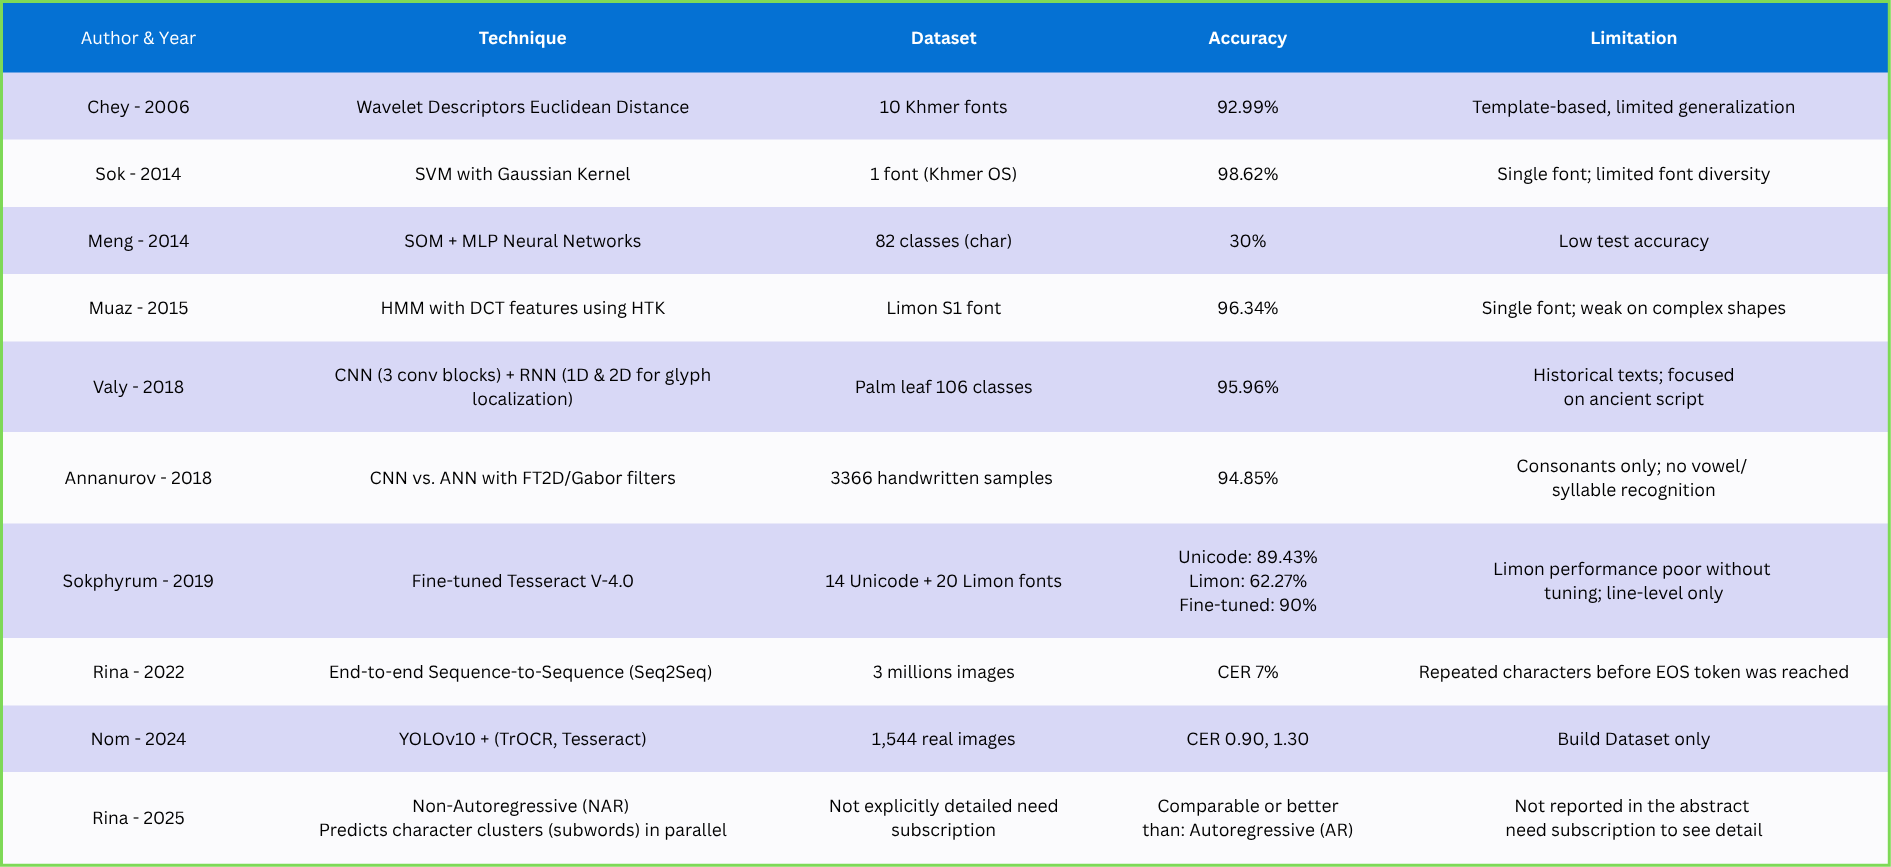
\includegraphics[width=\textwidth]{figures/summary_literature_review.png}
    \caption{Summary of the literature review, which includes the types of models used, 
    the datasets used, the metrics used to evaluate the performance of the models, 
    and the results of the experiments. The table highlights the key findings of the 
    literature review, including the challenges faced when developing Khmer OCR models 
    and the need for Khmer-specific models and datasets.}
    \label{fig:summary_literature_review}
\end{figure}

\section{Challenges in Khmer OCR}
\phantomsection
\label{sec:datasets}

Khmer OCR poses numerous technical challenges stemming from the script's unique structure and 
linguistic features. Unlike Latin-based scripts, Khmer characters can include complex stacking 
of consonants (e.g., subscript consonants using Coeng), placement of diacritics, and variable vowel 
positions that appear above, below, before, after, or even wrap around base characters \citep{buoy2021seq2seq}. 
This spatial complexity makes segmentation particularly difficult and often unreliable, 
especially in cluttered or noisy environments. Accurate character separation is further complicated 
by the fact that multiple elements can visually overlap, causing traditional segmentation-based 
approaches to fail.

Font diversity also adds a layer of complexity. Khmer is written using a wide array of fonts, each 
introducing variations in stroke thickness, character proportions, and spacing. These stylistic 
differences can drastically alter a character's appearance, requiring OCR systems to be highly 
font-invariant \citep{buoy2021seq2seq}. Yet, many models are trained on limited font sets, leading 
to poor generalization across unseen styles.

Another critical issue is the scarcity of annotated datasets. As a low-resource language, Khmer lacks 
the extensive labeled corpora available for Latin or Chinese scripts. This data scarcity hampers the 
training of robust models and forces researchers to rely on synthetic data or heavily augmented datasets 
to simulate real-world variability.

Additionally, many legacy OCR systems for Khmer rely on rule-based or modular pipelines with explicit 
character segmentation, manual pre- and post-processing, and assumptions about text structure. These 
approaches are brittle and poorly suited for real-world applications where scanned documents may contain 
noise, skew, blur, uneven lighting, or distorted text lines. Their reliance on handcrafted rules also 
limits scalability and adaptability to other domains.

Lastly, the lack of word boundaries in Khmer—where text is often written without spaces—presents an 
additional recognition barrier. This linguistic feature necessitates full line-level recognition, 
which increases computational complexity and requires models to understand broader contextual dependencies 
across characters.



\section{Role of Synthetic Data}
\phantomsection
\label{sec:dl-models}

To overcome the challenges associated with data scarcity in Khmer OCR, 
recent studies have emphasized the critical role of synthetic data generation. A prominent 
strategy involves leveraging the open-source \texttt{text2image} utility from the Tesseract OCR 
engine to create high-quality, rendered images of Khmer text lines \citep{buoy2021seq2seq}. 
These images are generated from a curated text corpus that includes a diverse mix of numbers, 
words, phrases, and full sentences, providing broad linguistic coverage.

Multiple commonly used Khmer fonts are applied during rendering to simulate font diversity and 
improve the model's ability to generalize across different typographic styles. Each rendered 
image is converted to grayscale and resized to a fixed height (e.g., 32 pixels) to meet the input 
dimensional requirements of neural network models, while maintaining proportional width to preserve 
text structure.

To emulate real-world conditions and enhance robustness, extensive data augmentation techniques 
are applied. These include Gaussian blurring, morphological operations like dilation and erosion, 
speckle and blob noise injection, background texture overlays, rotational distortions, and random 
concatenation of multiple text-line images. Each augmentation has a 50\% probability of being applied, 
with combinations occurring dynamically during training to maximize variability and minimize overfitting.

The resulting synthetic dataset scales to millions of samples, covering a wide spectrum of distortions, 
font styles, and text structures. This scale and diversity enable deep learning models—particularly 
end-to-end architectures such as attention-based Sequence-to-Sequence networks—to learn robust 
visual and contextual features, improving performance on both clean and noisy inputs. Ultimately, 
synthetic data serves as a vital resource for building Khmer OCR systems capable of handling the 
script’s inherent complexity in the absence of large, annotated real-world datasets.


\section{Summary of Research Gaps}
\phantomsection
\label{sec:research-gaps}

Despite recent progress in Khmer Optical Character Recognition (OCR), 
several critical gaps persist in the current body of research, hindering the 
development of robust and generalizable systems. First and foremost is the issue of 
data scarcity—there is a lack of large-scale, high-quality annotated datasets for Khmer, 
particularly for scene text and handwriting, which restricts model training, benchmarking, 
and cross-domain evaluation. Although synthetic datasets have partially mitigated this, they 
cannot fully replicate the variability and unpredictability of real-world documents. Second, the 
complex structural features of Khmer script—such as stacked consonants, overlapping vowel markers, and 
the absence of explicit word boundaries—are insufficiently addressed in many existing models, 
especially those adapted from Latin-script OCR frameworks. These models often fail to 
capture the script's spatial dependencies and morphological nuances. Third, font 
variability remains a major bottleneck: Khmer documents are written in a wide range of stylistic 
fonts, and OCR systems trained on limited font sets often generalize poorly. Lastly, there is 
a lack of robustness to real-world document conditions, including noisy backgrounds, image blur, 
skew, and low resolution. Many current systems, including Tesseract and some CNN-based models, 
show significant performance drops under such conditions. Addressing these gaps—through 
Khmer-specific model design, comprehensive dataset creation, and more resilient training strategies—is 
essential for building high-performance OCR systems tailored to the Khmer language and its 
real-world use cases.